\begin{appendices}

\chapter{Bayesian Optimization}

\begin{sidewaysfigure}[h]
\begin{subfigure}{\textwidth}
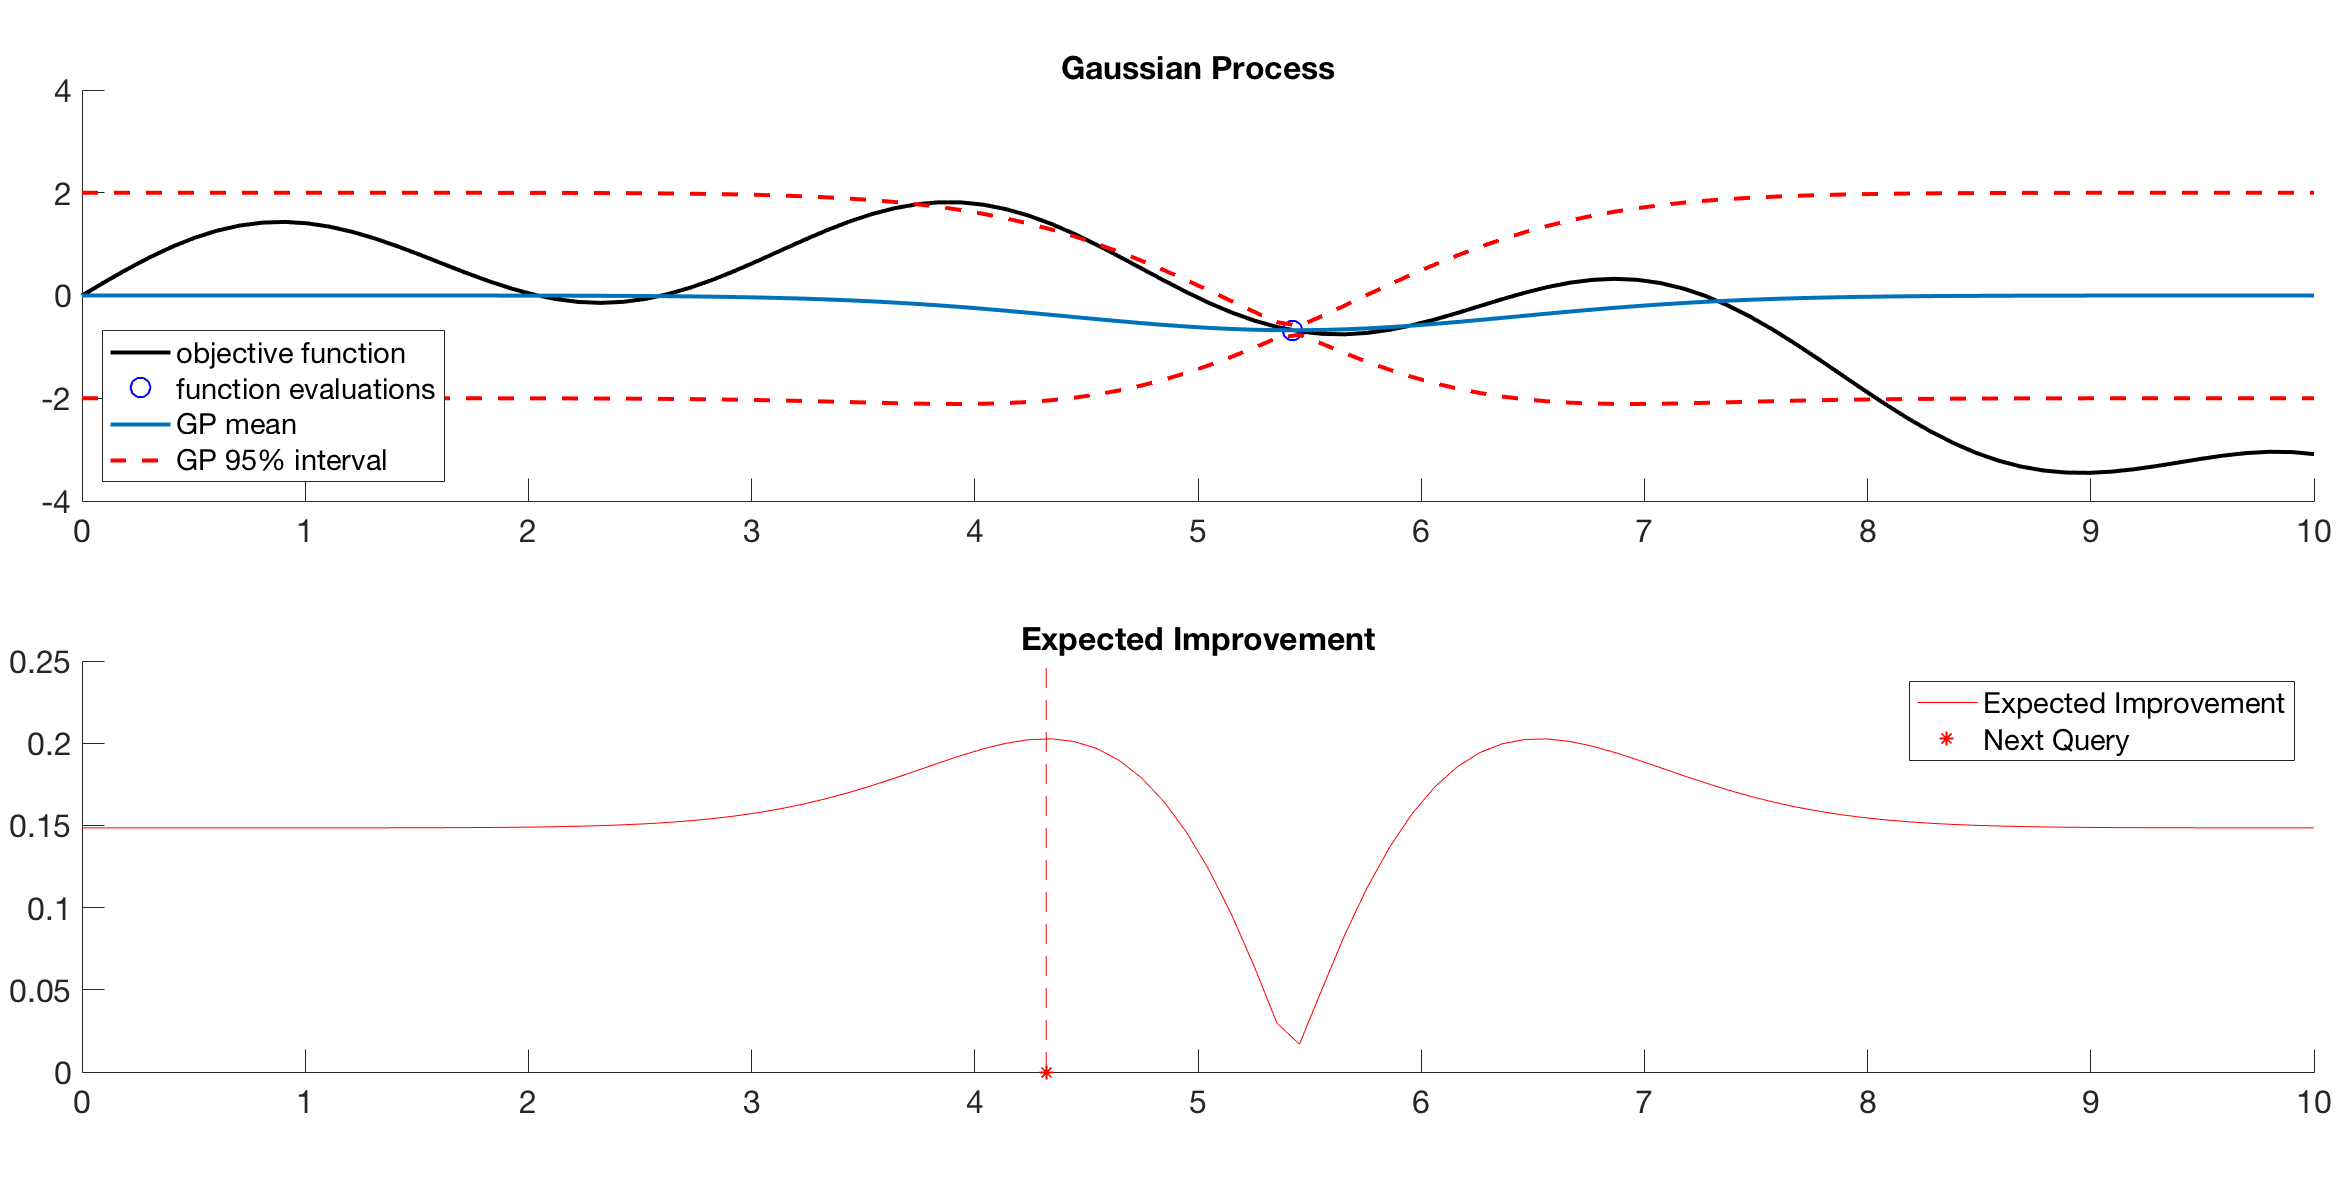
\includegraphics[width=.5\textwidth]{ei1.png}\hfill
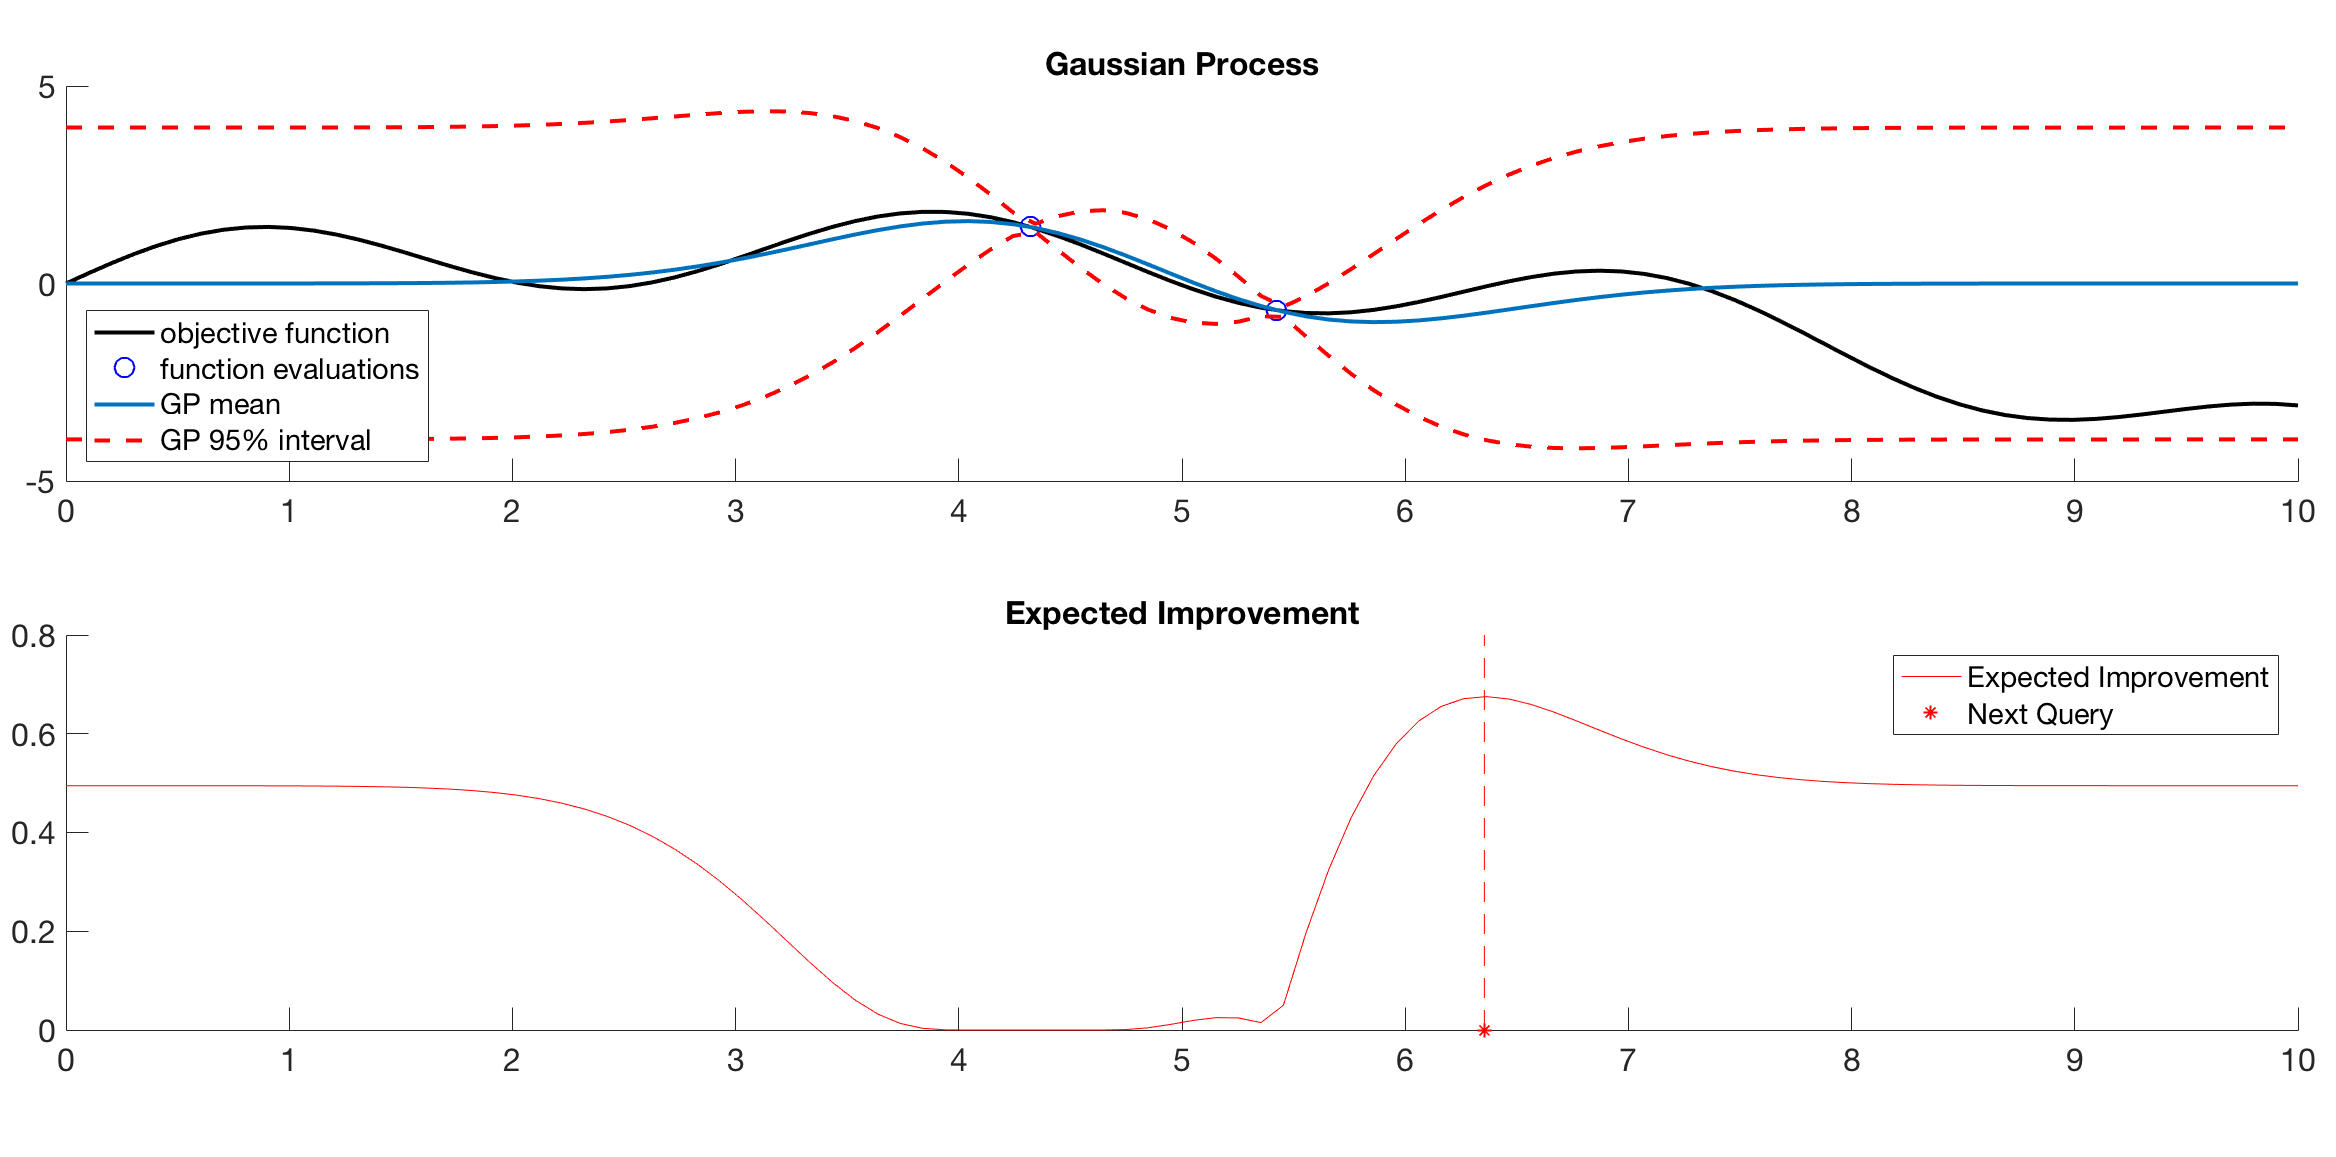
\includegraphics[width=.5\textwidth]{ei2.png}
\caption{Iterations 1 and 2}
\end{subfigure}
\par\medskip
\begin{subfigure}{\textwidth}
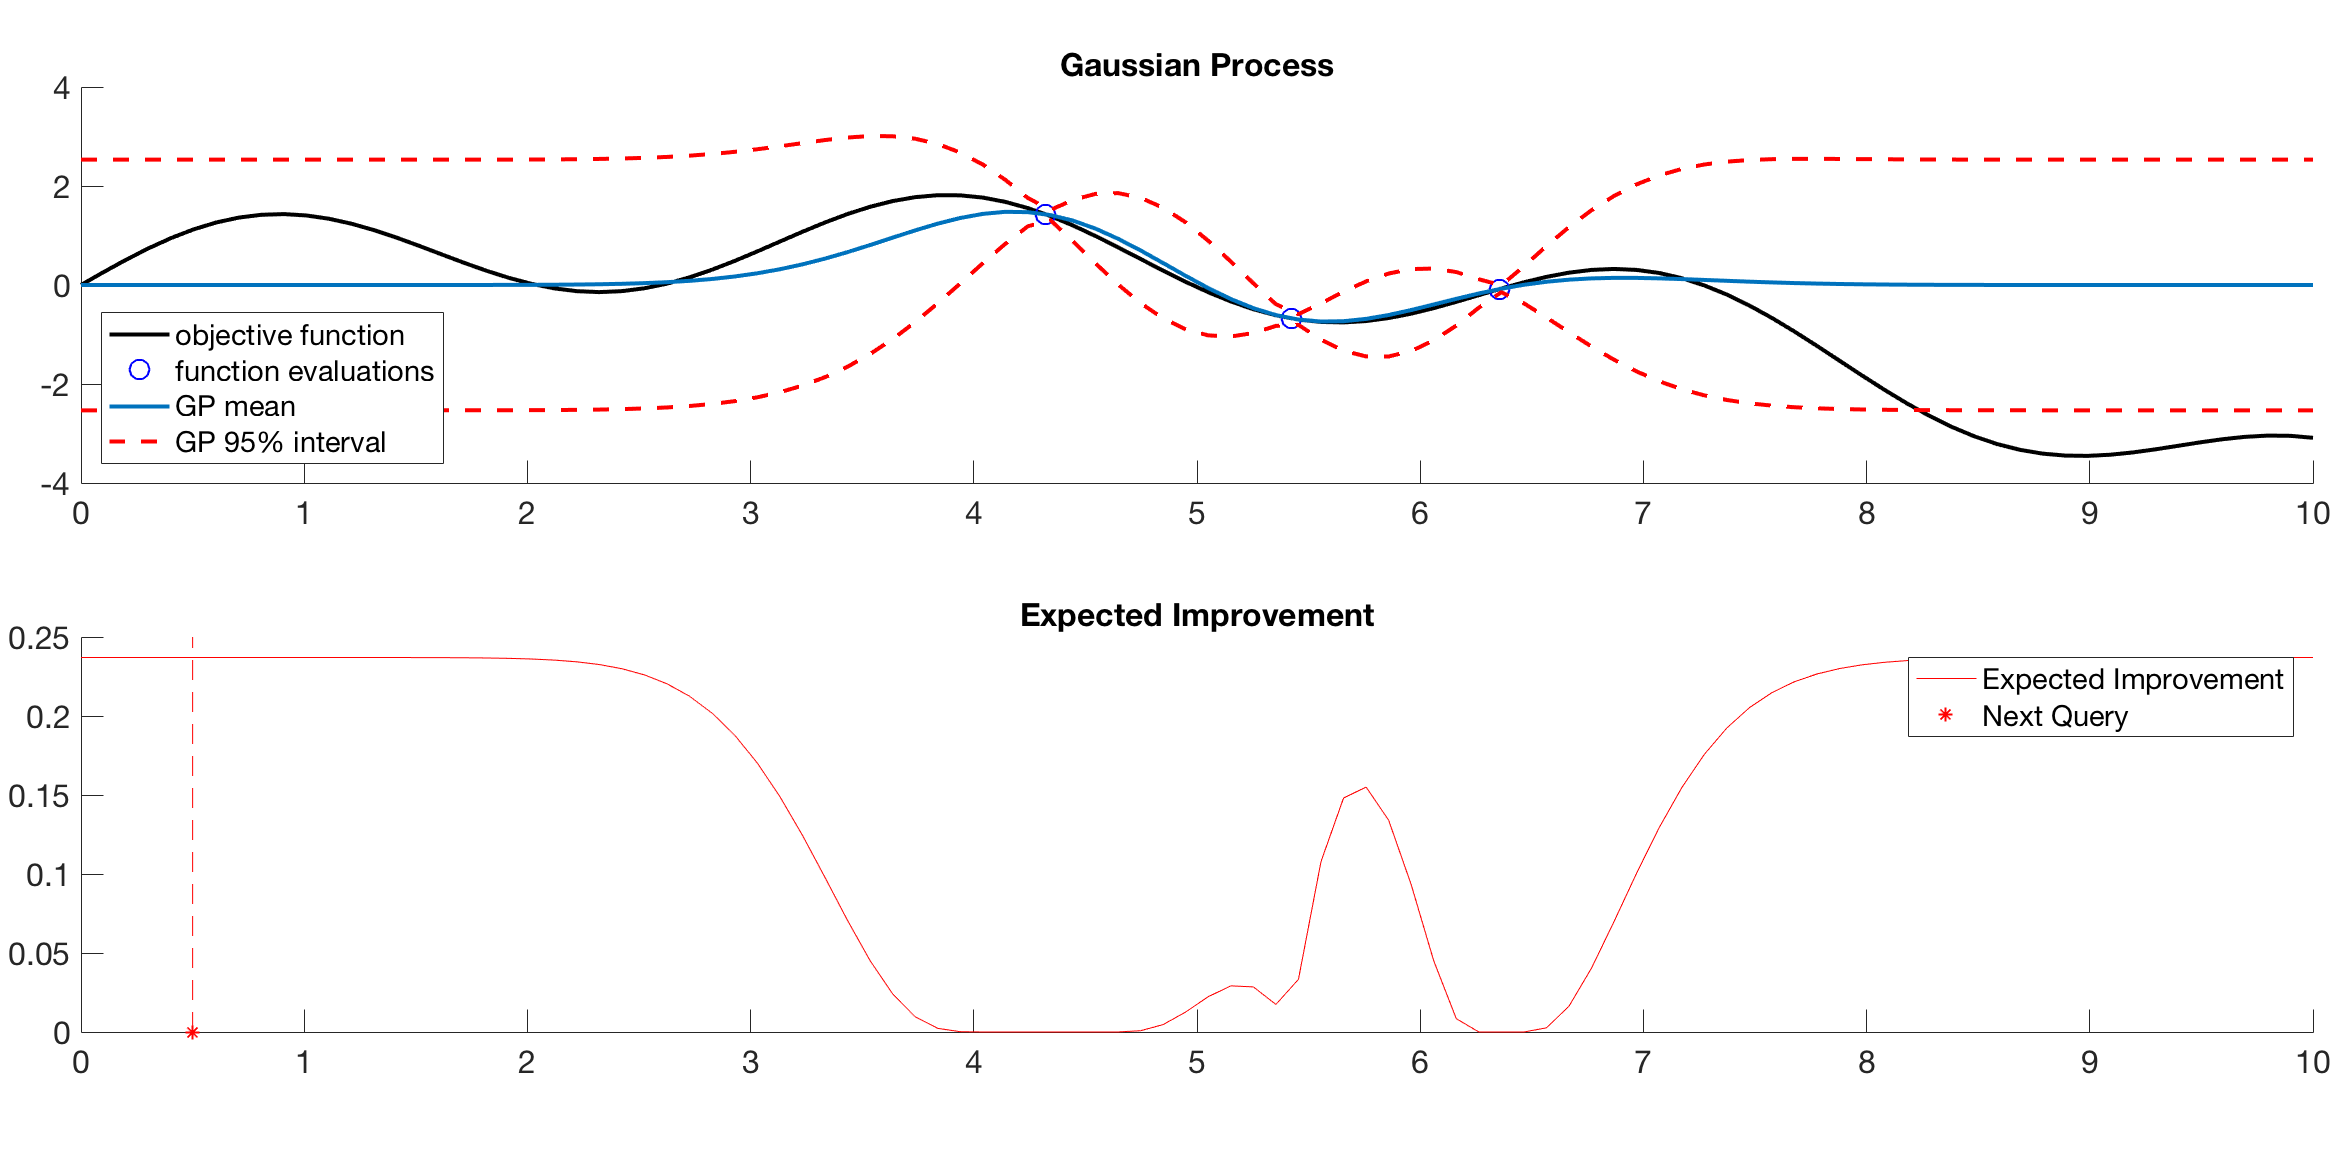
\includegraphics[width=.5\textwidth]{ei3.png}\hfill
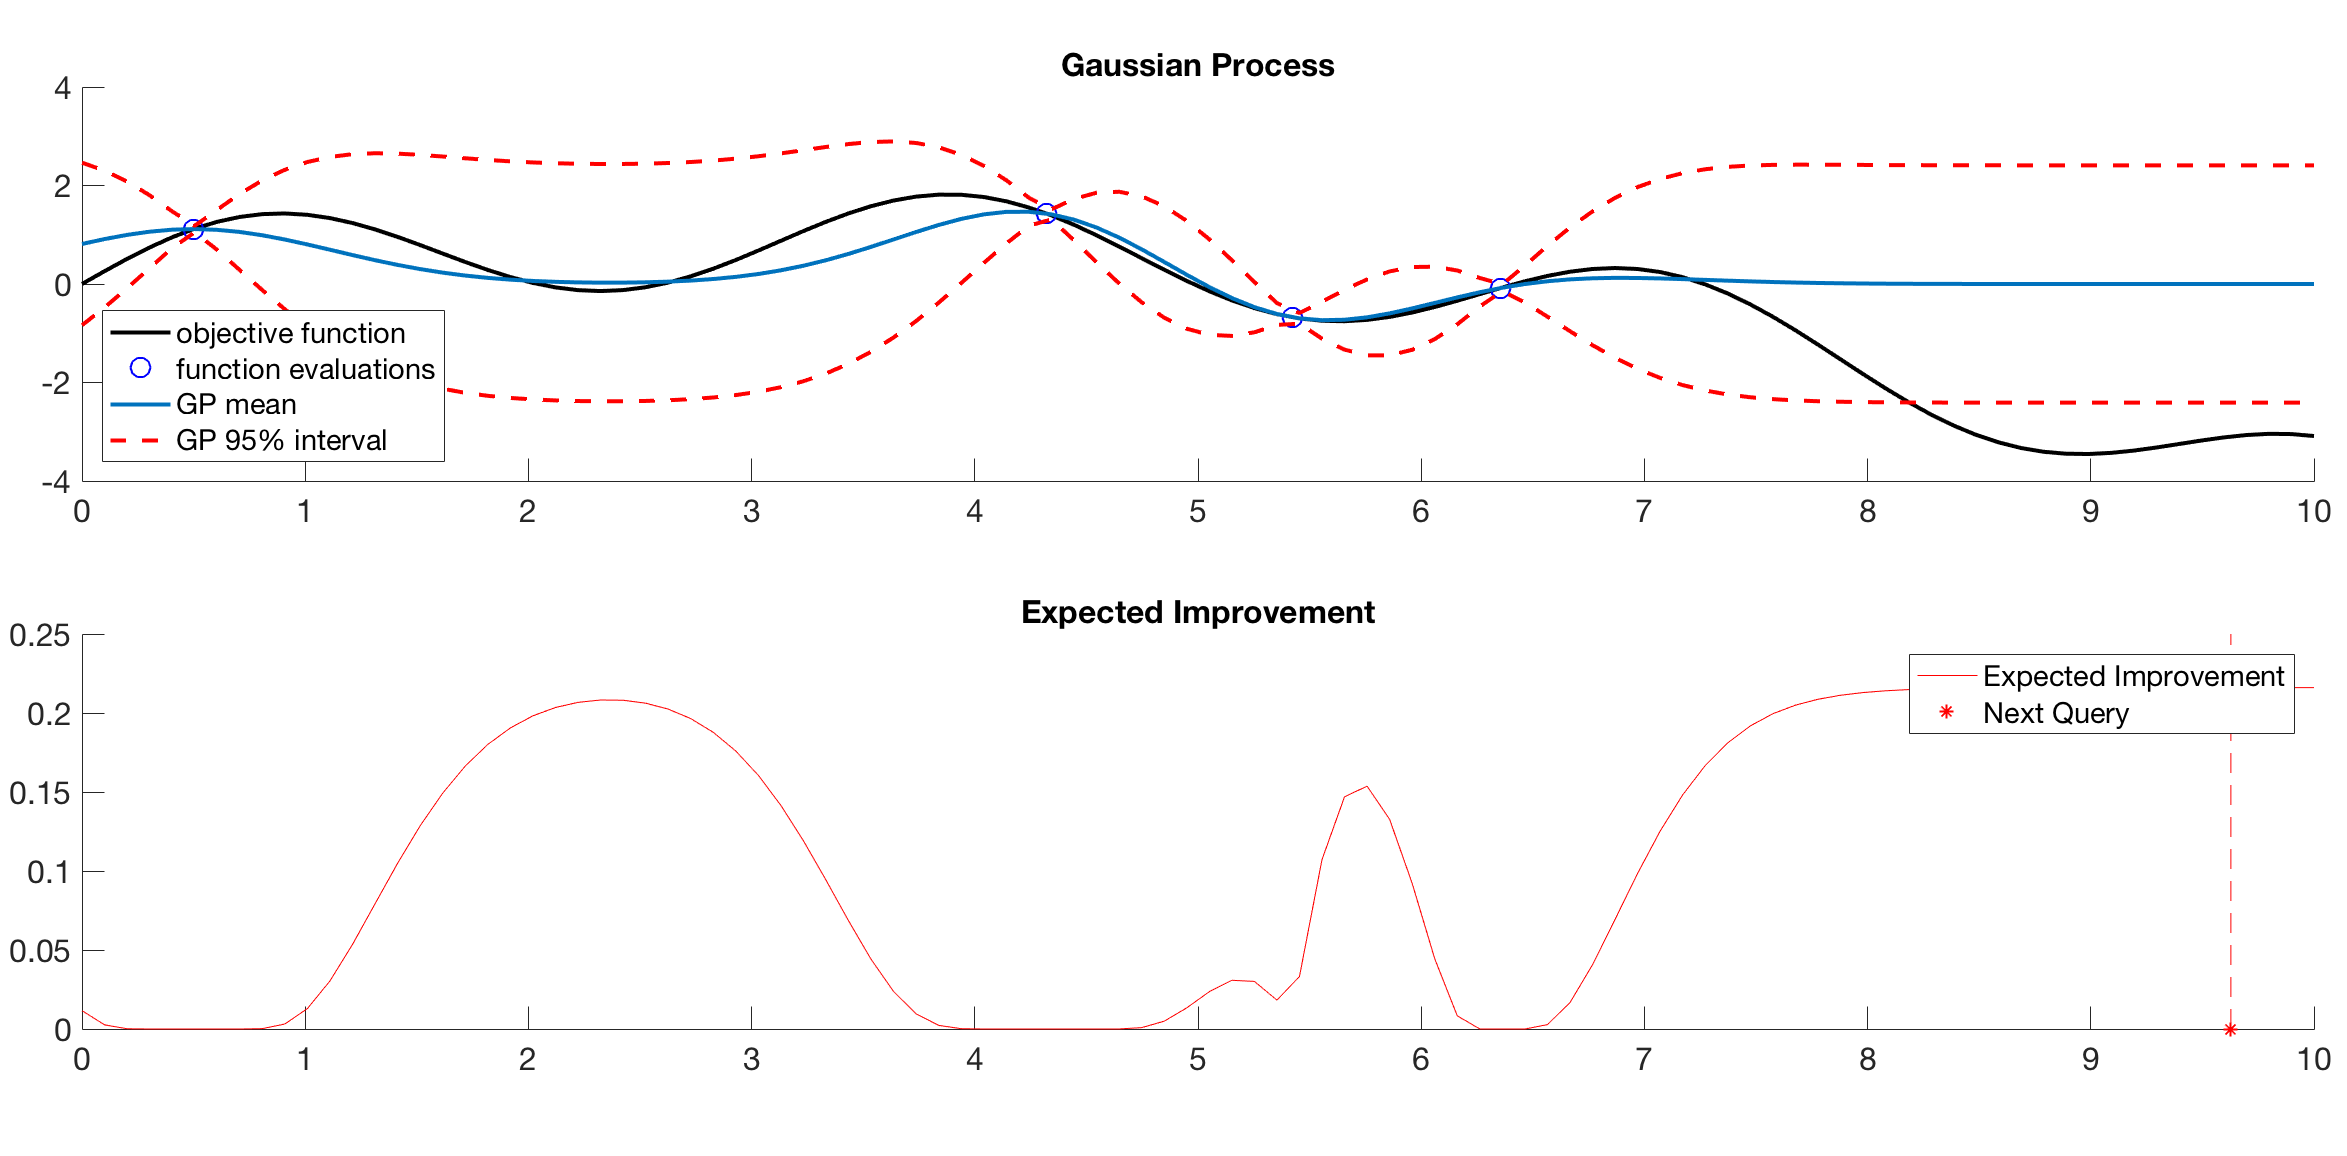
\includegraphics[width=.5\textwidth]{ei4.png}
\caption{Iterations 3 and 4}
\end{subfigure}
\caption{Four Iterations of Bayesian Optimization}
\label{fig:ei}
\end{sidewaysfigure}

%\chapter{Appendix to Chapter \ref{ch:2}}\label{cha:append-chapt-refch:2}
\chapter{Unscented Kalman Filter\footnote{\citet{Wan00theunscented}}}\label{sec:ukf}
The unscented transformation selects a representative set of points (sigma points) with associated weights to propagate through a nonlinear function. More formally, given an $N$-dimensional random variable $x$ with mean $\bar{x}$ and covariance $P_x$ we calculate the following sigma vectors 
\begin{equation}\label{eq:unscentedtransform}
\begin{aligned}
  \chi_0 &= \bar{x}\\
  \chi_i &= \bar{x} + (\sqrt{(N + \lambda)P_x})_i & i = 1, ..., N \\
  \chi_i &= \bar{x} - (\sqrt{(N + \lambda)P_x})_{i-N} & i = N + 1, ..., 2N\\
  W_0^{(m)} &= \lambda /(N + \lambda) \\
  W_0^{(c)} &= \lambda /(N + \lambda) + (1- \alpha^2 + \beta)\\
  W_i^m &= W_i^c = 1/\{(2(N + \lambda))\} & i = 1, ..., 2N,
\end{aligned}
\end{equation}
where $(\sqrt{(N + \lambda)P_x})_i$ represents the $i$th row of the matrix square root, $\lambda = \alpha^2(N + \kappa) - N$, and $\alpha$, $\kappa$, and $\beta$ are scaling parameters. For a given nonlinear function $y=g(x)$, an estimate for the mean and covariance are then
\begin{align}
\begin{split}
  \bar{y} &\approx \sum_{i=0}^{2N} W_i^{(m)}g(\chi_i)\\
  P_y &\approx \sum_{i=0}^{2N} W_i^{(c)}(g(\chi_i) - \bar{y})(g(\chi_i) - \bar{y})^T
\end{split}
\end{align}

Accurate to the second order, the Unscented Kalman Filter incorporates this transformation in it's $F$ and $H$ functions as follows:

\begin{algorithmic}
\State \textkeyword{Initial State Estimate and Covariance} $\hat{x}(0), P_{x}(0)$
\State \textkeyword{Define Augmented State } $x^a = [x^T \tab v^T \tab w^T]^T$
\State \textkeyword{Define Augmented Sigma Points } $\chi^a = [(\chi^x)^T  \tab (\chi^v)^T  \tab (\chi^w)^T]^T$
\State \textkeyword{Initial Augmented State Estimate } $\hat{x}^a(0) = [\hat{x}(0)^T  \tab 0  \tab 0]^T$
\State \textkeyword{Initial Augmented Covariance } $P^a(0) =
\begin{bmatrix}
	P_{x}(0) & 0 & 0\\
	0 & P_v & 0\\
	0 & 0 & P_w
\end{bmatrix}$ 
\For{t=1}{T}
  \State Using \ref{eq:unscentedtransform} Calculate Sigma Points $\chi^a(t)$ And Weights $W^{(m)}, W^{(c)}$
  \State Time Update:
  \begin{align*}
  	\chi_i^x(t\vert t-1) &= F(\chi_i^x(t-1), \chi_i^v(t-1), t-1)\\
  	\hat{x}(t\vert t-1) &= \sum_{i=0}^{2N} W_i^{(m)}\chi_i^x(t\vert t-1)\\
  	P_{x}(t\vert t-1) &= \sum_{i=1}^{2N} W_i^{(c)} \{\chi_i^x(t\vert t-1) - \hat{x}(t\vert t-1)\}\{\chi_i^x(t\vert t-1) - \hat{x}(t\vert t-1)\}^T\\
  	\mathbb{Z}_i(t\vert t-1) &= H(\chi_i^x(t\vert t-1), \chi_i^w(t-1), t-1)\\
  	\hat{z}(t\vert t-1) &= \sum_{i=1}^{2N} W_i^{(m)}\mathbb{Z}_i(t\vert t-1)
  \end{align*}
  \State Measurement Update:
  \begin{align*}
  	P_{y}(t\vert t-1) &= \sum_{i=1}^{2N}W_i^{(c)}\{\mathbb{Z}_i(t\vert t-1) - \hat{z}(t\vert t-1)\}\{\mathbb{Z}_i(t\vert t-1) - \hat{z}(t\vert t-1)\}^T\\
  	P_{xy}(t\vert t-1) &= \sum_{i=1}^{2N}W_i^{(c)}\{\chi_i^x(t\vert t-1) - \hat{x}(t\vert t-1)\}\{\chi_i^x(t\vert t-1) - \hat{x}(t\vert t-1)\}^T\\
  	K &= P_{xy}(t\vert t-1)P^{-1}_{y}(t\vert t-1)\\
  	\hat{x}(t) &= \hat{x}(t\vert t-1) + K(z(t) - \hat{z}(t\vert t-1))\\
  	P_{x}(t) &= P_{x}(t\vert t-1) - KP_{y}(t\vert t-1)K^T
  \end{align*}
\End
\end{algorithmic}

\chapter{Optimal Stopping Time Derivation}\label{thm:ost}
Define the process
\begin{align*}
	Z_n = \sum_{i=0}^{n-1} \lambda^ir(X_i) + \lambda^nJ_n(X_n)
\end{align*}
Then, we have
\begin{align*}
	\mathbb{E}[Z_{n+1} \vert X_n, X_{n-1}, ..., X_0] &= \sum_{i=0}^n \lambda^ir(X_i) + \lambda^{n+1}\mathbb{E}[J_{n+1}(X_{n+1})\vert X_n]\\
	&= \sum_{i=0}^{n-1} \lambda^ir(X_i) + \lambda^n(r(X_n) + \lambda\mathbb{E}[J_{n+1}(X_{n+1})\vert X_n])\\
	&\leq \sum_{i=0}^{n-1} \lambda^i r(X_i) + \lambda^nJ_n(X_n) = Z_n
\end{align*}
Since by definition $J_n(x) \geq g(x)$, we have
\begin{align*}
	\mathbb{E}[\sum_{i=0}^{\tau-1}\lambda^ir(X_i) + \lambda^{\tau}g(X_{\tau})] \leq \mathbb{E}[Z_{\tau}] \leq \mathbb{E}[Z_0] = J_0(X_0)
\end{align*}
for any stopping time $\tau \geq 0$. 

We now prove that $J_0(X_0)$ is exactly equal to $\mathbb{E}[Z_{\tau^*}]$ for optimal stopping time $\tau^*$. Consider the following for $0 \leq n < N$
\begin{align*}
	\mathbb{E}&[Z_{min(\tau^*, n+1)}\vert X_n, X_{n-1}, ..., X_0]\\
	&= 1_{\{\tau^* \leq n\}}Z_{\tau^*} + 1_{\{\tau^* > n\}}\mathbb{E}[Z_{n+1}\vert X_n, X_{n-1}, ..., X_0]\\
	&= 1_{\{\tau^* \leq n\}}Z_{\tau^*} + 1_{\{\tau^* > n\}}(\sum_{i=0}^n \lambda^ir(X_i) + \lambda^{n+1}\mathbb{E}[J_{n+1}(X_{n+1})\vert X_n])\\
	&= 1_{\{\tau^* \leq n\}}Z_{\tau^*} + 1_{\{\tau^* > n\}}(\sum_{i=0}^{n-1} \lambda^ir(X_i) + \lambda^nJ_n(X_n)) \tab (\tau^* > n\leftrightarrow J_n(X_n) = r(x) + \lambda\mathbb{E}[J_{n+1}(X_{n+1})])\\ 
	&= 1_{\{\tau^* \leq n\}}Z_{\tau^*} + 1_{\{\tau^* > n\}}Z_{n}\\
	&= Z_{min(\tau^*, n)}
\end{align*}
Then, it follows that
\begin{align*}
	J_0(X_0) &= \mathbb{E}[Z_0] = \mathbb{E}[Z_{min(\tau^*, 0)}] = ... = \mathbb{E}[Z_{min(\tau^*, N)}] = \mathbb{E}[Z_{\tau^*}]\\
			 &= \mathbb{E}[\sum_{i=0}^{\tau^* -1}\lambda^ir(X_i) + \lambda^{\tau^*}J_{\tau^*}(X_{\tau^*})] = \mathbb{E}[\sum_{i=0}^{\tau^* -1}\lambda^ir(X_i) + \lambda^{\tau^*}g(X_{\tau^*})]
\end{align*}
and $J_{\tau^*}(X_{\tau^*}) = g(X_{\tau^*})$ at $\tau^*$.
\end{appendices}
